\chapter{Optymalizacja kosztu gazu w warstwie pierwszej}
\label{ch:gaz}

Rozdział bada, jak decyzje projektowe wpływają na koszt gazu kontraktu rejestru
dyplomów na Ethereum. Eksperymenty podzielono na trzy etapy, każdy odpowiadający
innemu poziomowi abstrakcji decyzji: (1)~mikrooptymalizacje modelu per-dyplom ---
siedem kolejnych wersji kontraktu z~pojedynczymi zmianami kodu; (2)~zmianę
architektury na \emph{Merkle batch}, w~której jedna transakcja pokrywa całą partię;
(3)~mikrooptymalizacje hot-path weryfikacji dowodu Merkle. Wnioski z~trzech
etapów zbiera sekcja~\ref{sec:gaz-wnioski}.

\section{Metodyka pomiaru}
\label{sec:gaz-metodyka}

Wszystkie pomiary wykonano lokalnie w~środowisku Foundry~\cite{foundry}
(Solidity 0.8.20), co eliminuje szum wynikający ze zmienności opłat sieciowych. Foundry dostarcza dwie
granulacje danych:

\begin{itemize}
  \item \textbf{Suite-level} --- łączny gaz jednego testu, włącznie z~setupem
        (deploy kontraktu, wywołania przygotowawcze). Oddaje realistyczny koszt
        całego scenariusza.
  \item \textbf{Function-level} (\code{--gas-report}) --- gaz samej funkcji EVM,
        agregowany po wszystkich jej wywołaniach w~suite jako min/avg/max. Pozwala
        precyzyjnie izolować koszt jednej operacji.
\end{itemize}

\noindent Komendy użyte do pomiarów:
\begin{verbatim}
cd contracts
forge test --match-path "test/DiplomaRegistry[ABCDEF]*.t.sol" --gas-report
forge test --match-path "test/DiplomaRegistryGasComparison.t.sol" --gas-report
\end{verbatim}

\section{Etap 1 --- mikrooptymalizacje modelu per-dyplom}
\label{sec:gaz-etap1}

Model per-dyplom to najprostsze możliwe podejście: każdy dyplom to jeden wpis
\code{mapping(bytes32 => Record)}. Zbadano siedem kolejnych wersji kontraktu, aby
sprawdzić, jak bardzo zmiana jednej konkretnej decyzji implementacyjnej wpływa na
koszt gazu. Wersjom nadano nazwy opisujące \emph{kluczową właściwość}
odróżniającą każdą z~nich od poprzedniej.

\subsection{Wersje kontraktu}

\begin{table}[H]
\centering
\caption{Chronologiczne wersje kontraktu per-dyplom: zakres i~uzasadnienie zmian.}
\begin{tabular}{>{\bfseries}p{3.0cm}
                >{\raggedright\arraybackslash}p{4.5cm}
                >{\raggedright\arraybackslash}p{6.5cm}}
\toprule
Nazwa wersji & Kluczowa zmiana & Uzasadnienie / hipoteza \\
\midrule
\code{StringErrors}
  & \code{require(..., "STRING")}, \newline rekord: \code{\{issuer, issuedAt, revoked\}}, \newline mutable \code{owner}
  & Punkt startowy --- kontrakt pisany intuicyjnie, bez optymalizacji \\[6pt]

\code{TimestampRevoke}
  & \code{revokedAt(uint64)} zamiast \code{bool}
  & Hipoteza: timestamp rewokacji przyda się audytorom; \newline \textbf{efekt: regres} --- dodatkowy slot storage \\[6pt]

\code{CustomErrors}
  & \code{custom errors} zamiast komunikatów string
  & Komunikaty string są kodowane jako dane, \newline custom errors to 4-bajtowy selektor \\[6pt]

\code{ImmutableOwner}
  & \code{owner} jako \code{immutable}
  & \code{immutable} trzyma wartość w~bytecode, \newline nie w~storage --- brak odczytu SLOAD w~modyfikatorze \\[6pt]

\code{Idempotent}
  & \code{addIssuer}/\code{removeIssuer} nie rzucają przy ponownym wywołaniu
  & Zabezpieczenie przed kosztownym revert-em \newline w~przypadku race condition \\[6pt]

\code{MinimalRecord}
  & Usunięcie timestampów ze storage; \newline rekord: \code{\{issuer, revoked\}}
  & Daty pozostają dostępne w~logach zdarzeń; \newline duplikacja w~storage jest zbędna \\[6pt]

\code{PackedStorage}
  & \code{mapping(bytes32 => uint256)}: \newline issuer (160 bitów) + bit revoked \newline w~jednym slocie; dodano \code{status()}
  & Jeden SLOAD zamiast dwóch --- rozkład adresu \newline i~flagi z~jednej 256-bitowej wartości \\
\bottomrule
\end{tabular}
\end{table}

\subsection{Wyniki}

Poniższa tabela pokazuje łączny koszt jednego scenariusza testowego (suite-level).
Warto pamiętać, że \code{testGas\_revoke} zawiera wywołanie \code{issue} jako setup
stanu --- dlatego wartości w~tej kolumnie są wyższe niż sam koszt rewokacji.

\begin{table}[H]
\centering
\caption{Koszt testów end-to-end w~gazie, łącznie z~deployem i~setupem (kolumny to
warianty \code{testGas\_addIssuer}, \code{testGas\_issue}, \code{testGas\_revoke}).}
\begin{tabular}{l r r r >{\raggedright\arraybackslash}p{3.1cm}}
\toprule
Wersja & \code{addIssuer} & \code{issue} & \code{revoke} & Uwagi \\
\midrule
\code{StringErrors}    & 57\,119 & 60\,721 &  93\,116 & punkt startowy \\
\code{TimestampRevoke} & 57\,153 & 62\,890 & 114\,348 & \textbf{regres: +21k gas na revoke} \\
\code{CustomErrors}    & 57\,186 & 63\,012 & 114\,380 & pozornie bez poprawy (por.\ function-level) \\
\code{ImmutableOwner}  & 55\,100 & 63\,037 & 114\,431 & drobna poprawa addIssuer \\
\code{Idempotent}      & 55\,312 & 63\,047 & 114\,448 & marginalnie droższy w~tym scenariuszu \\
\code{MinimalRecord}   & 55\,100 & 60\,569 &  92\,868 & powrót do taniego \code{revoke} \\
\code{PackedStorage}   & 55\,056 & 60\,531 &  92\,797 & najlepszy wynik ogólny \\
\bottomrule
\end{tabular}
\end{table}

\noindent Najistotniejszą obserwacją jest \textbf{regres w~wersji
\code{TimestampRevoke}}: dodanie pola \code{uint64 revokedAt} do rekordu zwiększa
koszt rewokacji z~93k do 114k gas, ponieważ EVM musi zaktualizować dodatkowy slot
storage przy każdym \code{revoke()}. Wersja \code{MinimalRecord} naprawia ten błąd,
usuwając timestampy ze storage i~pozostawiając je wyłącznie w~logach zdarzeń.

Widok function-level pozwala zmierzyć czysty koszt każdej operacji, niezależnie od
kontekstu testu. Różnice deployment są tutaj bardziej widoczne niż w~suite-level.

\begin{table}[H]
\centering
\caption{Koszt deploymentu i~średni koszt operacji wg \code{forge --gas-report} (Avg).}
\begin{tabular}{lrrrr}
\toprule
Wersja & Deployment & \code{addIssuer} & \code{issue} & \code{revoke} \\
\midrule
\code{StringErrors}    & 464\,211 & 45\,719 & 48\,458 & 31\,274 \\
\code{TimestampRevoke} & 469\,181 & 46\,963 & 50\,659 & 50\,369 \\
\code{CustomErrors}    & 409\,497 & 45\,904 & 43\,367 & 38\,867 \\
\code{ImmutableOwner}  & 403\,109 & 43\,366 & 43\,370 & 38\,870 \\
\code{Idempotent}      & 418\,029 & 43\,523 & 43\,377 & 38\,874 \\
\code{MinimalRecord}   & 373\,484 & 43\,366 & 41\,607 & 28\,825 \\
\code{PackedStorage}   & 393\,596 & 43\,621 & 43\,084 & 29\,302 \\
\bottomrule
\end{tabular}
\end{table}

\noindent Widok function-level ujawnia efekt niewidoczny na poziomie suite:
\code{CustomErrors}
redukuje deployment z~464k do 409k gas, ponieważ komunikaty string (\code{"Only owner"},
\code{"Already issued"}, itd.) są przechowywane w~bytecode kontraktu, a~\code{custom
errors} zastępuje je 4-bajtowymi selektorami. Ta zmiana oszczędza \emph{rozmiar
kodu}, co przekłada się na tańszy deployment: redukcja o~55\,000 gas (11{,}9\%).

Nie każda zmiana poprawia sytuację --- \code{TimestampRevoke} jest przykładem
modyfikacji wprowadzonej w~dobrej intencji, której koszt znacząco przewyższył
oczekiwania: przechowywanie znacznika czasu rewokacji w~storage zamiast
w~zdarzeniach zwiększyło koszt \code{revoke} o~61\%. Sumarycznie, od \code{StringErrors} do \code{MinimalRecord}:
\[
  \Delta_{\code{issue}} \approx 14{,}1\%,\quad
  \Delta_{\code{revoke}} \approx 7{,}8\%,\quad
  \Delta_{\text{deploy}} \approx 19{,}6\%.
\]

\section{Etap 2 --- architektura Merkle batch}
\label{sec:gaz-etap2}

Model per-dyplom zakłada, że \emph{każdy dyplom trafia na łańcuch jako osobna
transakcja}. Architektura Merkle batch znosi to założenie: zamiast zapisywać $N$
dyplomów w~$N$ transakcjach, wystawca:
\begin{enumerate}
  \item buduje drzewo Merkle z~$N$ liści (off-chain, bez gazu),
  \item zapisuje na łańcuch wyłącznie \textbf{korzeń drzewa} --- jedną transakcję
        \code{issueBatchRoot(batchId, merkleRoot)},
  \item weryfikacja dyplomu przez \code{statusWithProof(docHash, issuer, batchId,
        proof)} sprawdza przynależność liścia do korzenia, używając dowodu
        $O(\log N)$.
\end{enumerate}

\subsection{Zmiana modelu operacji}

\begin{table}[H]
\centering
\caption{Mapowanie operacji: model per-dyplom (\code{PackedStorage}) vs Merkle.}
\begin{tabular}{p{3.5cm} p{4.5cm} p{5.5cm}}
\toprule
Operacja & \code{PackedStorage} (per-dyplom) & \code{MerkleBaseline} \\
\midrule
Wystawienie & \code{issue(docHash)} --- 1 tx / dyplom & \code{issueBatchRoot(batchId, root)} --- 1 tx / N dyplomów \\[4pt]
Weryfikacja & \code{status(docHash)} --- odczyt mapping & \code{statusWithProof(hash, issuer, batchId, proof)} --- weryfikacja Merkle \\[4pt]
Rewokacja & \code{revoke(docHash)} --- prosty SSTORE & \code{revokeFromBatch(hash, batchId, proof)} --- SSTORE + weryfikacja \\[4pt]
Zarządzanie \newline wystawcami & \code{addIssuer}/\code{removeIssuer} & \code{onboardIssuerAndUniversity} (bogatszy model z~uczelnią) \\
\bottomrule
\end{tabular}
\end{table}

\subsection{Wyniki: koszt na dyplom}

\begin{table}[H]
\centering
\caption{\code{PackedStorage} vs \code{MerkleBaseline} --- min/avg/max wg \code{forge --gas-report}.}
\begin{tabular}{llrrr}
\toprule
Model & Operacja & Min & Avg & Max \\
\midrule
\multirow{4}{*}{\code{PackedStorage}} &
  \code{addIssuer}    & 21\,585 & 43\,621 & 44\,855 \\
& \code{issue}        & 24\,030 & 43\,084 & 48\,200 \\
& \code{removeIssuer} & 21\,607 & 23\,112 & 24\,947 \\
& \code{revoke}       & 26\,407 & 29\,302 & 31\,222 \\
\midrule
\multirow{4}{*}{\code{MerkleBaseline}} &
  \code{issueBatchRoot}  & 50\,927 & 50\,937 & 50\,939 \\
& \code{revokeFromBatch} & 54\,239 & 57\,229 & 61\,591 \\
& \code{statusWithProof} & 10\,555 & 11\,890 & 13\,835 \\
& \code{onboardIssuer\&Uni} & \multicolumn{3}{c}{76\,907 (stałe)} \\
\midrule
\multicolumn{2}{l}{Deployment} & \multicolumn{2}{l}{\code{PackedStorage}: 393\,596} & \\
\multicolumn{2}{l}{} & \multicolumn{2}{l}{\code{MerkleBaseline}: 1\,059\,364 ($\times$2{,}7)} & \\
\bottomrule
\end{tabular}
\end{table}

\noindent Na poziomie pojedynczej transakcji Merkle nie jest tańszy ---
\code{issueBatchRoot} kosztuje tyle samo co \code{issue} w~per-dyplom. Właściwą
metryką porównania jest jednak \textbf{koszt na dyplom}, ponieważ jedna
transakcja \code{issueBatchRoot} obejmuje $N$ dyplomów:
\[
  \text{gas\_per\_diploma}(N) = \frac{50\,939}{N},
  \qquad
  \text{gas\_per\_diploma}_\text{legacy} = 48\,200 = \text{const}.
\]

\begin{figure}[H]
\centering
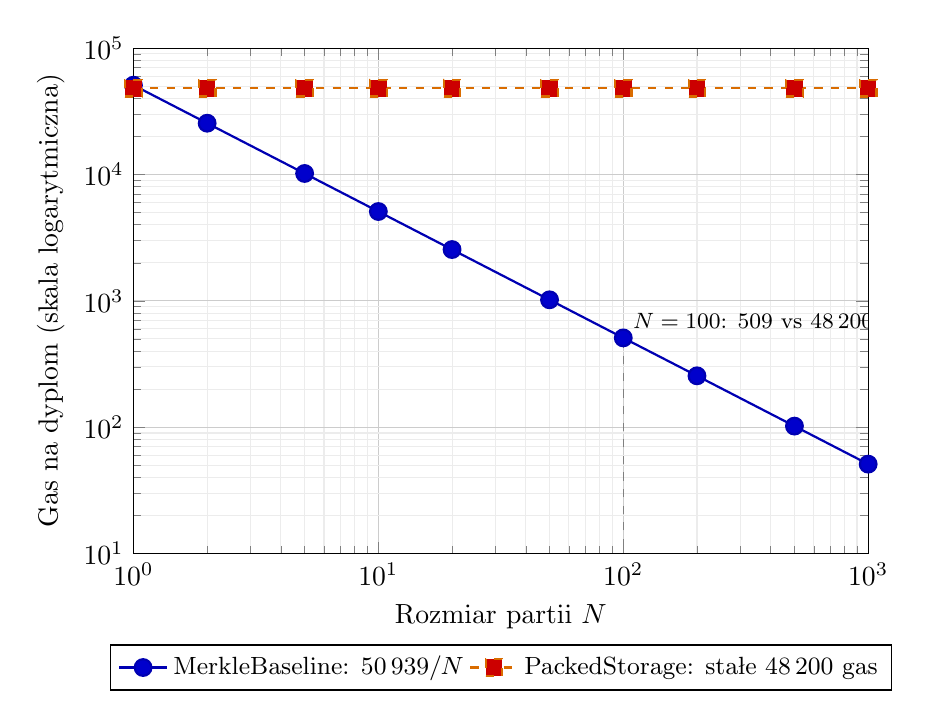
\begin{tikzpicture}
\begin{axis}[
    width=0.90\textwidth,
    height=8cm,
    xlabel={Rozmiar partii $N$},
    ylabel={Gas na dyplom (skala logarytmiczna)},
    xmode=log, ymode=log,
    log basis x={10}, log basis y={10},
    xmin=1, xmax=1000,
    ymin=10, ymax=100000,
    grid=both,
    minor grid style={gray!15},
    major grid style={gray!40},
    legend style={at={(0.5,-0.18)},anchor=north,font=\small},
    legend columns=2,
]
\addplot+[mark=*, thick, color=blue!70!black, mark size=3pt]
  coordinates {(1,50939)(2,25469)(5,10188)(10,5094)(20,2547)
               (50,1019)(100,509)(200,255)(500,102)(1000,51)};
\addlegendentry{\code{MerkleBaseline}: $50\,939/N$}
\addplot+[mark=square*, thick, color=orange!85!black, dashed, mark size=3pt]
  coordinates {(1,48200)(2,48200)(5,48200)(10,48200)(20,48200)
               (50,48200)(100,48200)(200,48200)(500,48200)(1000,48200)};
\addlegendentry{\code{PackedStorage}: stałe 48\,200 gas}
\draw[dashed,gray] (axis cs:100,1) -- (axis cs:100,509);
\node[anchor=south west, font=\footnotesize] at (axis cs:100,509)
  {$N=100$: $509$ vs $48\,200$};
\end{axis}
\end{tikzpicture}
\caption[Amortyzacja kosztu publikacji: legacy vs Merkle batch]{Amortyzacja kosztu publikacji: model Merkle obniża koszt na dyplom
odwrotnie proporcjonalnie do rozmiaru partii $N$, podczas gdy w~modelu
per-dyplom koszt jest stały; próg opłacalności leży już przy $N \approx 1$
(skala logarytmiczna na obu osiach).}
\end{figure}

\begin{table}[H]
\centering
\caption{Konkretne wartości: gas na dyplom i~stosunek do modelu legacy.}
\begin{tabular}{rrrr}
\toprule
$N$ & Merkle (gas/dyplom) & Legacy (gas/dyplom) & Krotność redukcji \\
\midrule
1    & 50\,939 & 48\,200 & $0{,}95\times$ (legacy tańszy) \\
5    & 10\,188 & 48\,200 & $4{,}7\times$ \\
10   &  5\,094 & 48\,200 & $9{,}5\times$ \\
50   &  1\,019 & 48\,200 & $47\times$ \\
100  &    509  & 48\,200 & $\mathbf{94{,}7\times}$ \\
500  &    102  & 48\,200 & $472\times$ \\
1000 &     51  & 48\,200 & $945\times$ \\
\bottomrule
\end{tabular}
\end{table}

\noindent Przejście na Merkle to \emph{nie kolejna mikrooptymalizacja} --- to inna
odpowiedź na pytanie o~model danych. Koszt jednostkowej transakcji jest taki sam jak
legacy (lub nawet minimalnie wyższy), ale pojedyncza transakcja ,,certyfikuje'' całą
partię. Przy $N=100$ koszt per dyplom spada z~$\approx$48\,200 do $\approx$509 gas
--- \textbf{redukcja o 98{,}9\%}. Ceną za tę zmianę jest niemal trzykrotnie droższy
deployment ($\approx$1{,}06M vs $\approx$0{,}39M gas) oraz bardziej złożona weryfikacja
wymagająca dowodu Merkle.

\section{Etap 3 --- optymalizacje hot-path Merkle}
\label{sec:gaz-etap3}

Po wyborze architektury Merkle pozostaje pytanie, czy ścieżkę weryfikacji dowodu
można dalej zoptymalizować na poziomie kodu EVM. Kontrakt
\code{DiplomaRegistryG} (dalej: \code{MerkleG}) to identyczny funkcjonalnie wariant
\code{MerkleBaseline} z~czterema przyrostowymi technikami nałożonymi na dwie
wewnętrzne funkcje: \code{\_processProof()} (iteracja po elementach dowodu)
i~\code{\_merkleLeaf()} (budowanie liścia do zhashowania).

\subsection{Techniki G1--G4}

Tabela~\ref{tab:g1g4} zestawia cztery zastosowane techniki wraz z~miejscem ich
działania i~mechanizmem oszczędności.

\begin{table}[H]
\centering
\caption{Cztery techniki zastosowane w~\code{MerkleG}.}
\label{tab:g1g4}
\begin{tabular}{>{\bfseries}p{2.8cm} p{4.0cm} p{7.0cm}}
\toprule
Nazwa & Gdzie & Co robi i~dlaczego oszczędza gas \\
\midrule
G1 \newline \code{unchecked++i}
  & \code{\_processProof}, pętla
  & Blok \code{unchecked\{\}} eliminuje sprawdzanie przepełnienia licznika
    iteracji; pre-increment \code{++i} zamiast \code{i++} nie tworzy kopii. Razem:
    kilka opcodów mniej na krok. \\[4pt]

G2 \newline assembly keccak
  & \code{\_processProof}, krok haszowania
  & Hashowanie pary liści przez \code{keccak256(0x00, 0x40)} --- dane pisane
    bezpośrednio do \emph{scratch space} EVM (bajty 0x00--0x3f), który istnieje
    zawsze i~nie wymaga aktualizacji wskaźnika wolnej pamięci
    (\code{mload/mstore 0x40}). Eliminuje alokację pamięci na każdym kroku pętli. \\[4pt]

G3 \newline prywatny liść
  & \code{\_merkleLeaf}, ścieżka wewnętrzna
  & Publiczny \code{merkleLeaf()} weryfikuje, że \code{docHash != 0} i~\code{issuer
    != 0}. Prywatne \code{\_merkleLeaf()} te sprawdzenia pomija --- bo kod
    wywołujący je wcześniej już zweryfikował dane. Oszczędność: dwa warunkowe rzuty
    mniej. \\[4pt]

G4 \newline assembly \mbox{preimage}
  & \code{\_merkleLeaf}, budowanie danych
  & Zamiast \code{abi.encodePacked(address(this), chainid(), issuer, batchId,
    docHash)} (112 bajtów, alokacja przez ABI-encoder), dane pakowane są przez
    ręczne \code{mstore} z~przesunięciami bitowymi. Oszczędność: cały narzut
    ABI-encodera na budowanie 112-bajtowego bufora. \\
\bottomrule
\end{tabular}
\end{table}

\subsection{Wyniki}

\begin{table}[H]
\centering
\caption{\code{MerkleBaseline} vs \code{MerkleG} --- min/avg/max wg Foundry.}
\begin{tabular}{lrrrrrrc}
\toprule
Operacja
  & \multicolumn{3}{c}{\code{MerkleBaseline}}
  & \multicolumn{3}{c}{\code{MerkleG}}
  & $\Delta$ Avg \\
\cmidrule(lr){2-4}\cmidrule(lr){5-7}
& Min & Avg & Max & Min & Avg & Max & \\
\midrule
Deployment
  & \multicolumn{3}{c}{1\,059\,364}
  & \multicolumn{3}{c}{1\,018\,273}
  & $-41\,091$ (\textbf{$-$3{,}9\%}) \\
\code{issueBatchRoot}
  & 50\,927 & 50\,937 & 50\,939
  & 50\,927 & 50\,937 & 50\,939
  & $0$ \\
\code{revokeFromBatch}
  & 54\,239 & 57\,229 & 61\,591
  & 54\,101 & 56\,443 & 59\,859
  & $-786$ ($-1{,}4\%$) \\
\code{statusWithProof}
  & 10\,555 & 11\,890 & 13\,835
  & 10\,417 & 11\,104 & 12\,103
  & $-786$ (\textbf{$-$6{,}6\%}) \\
\code{merkleLeaf} (view)
  & 866 & 866 & 866
  & 824 & 824 & 824
  & $-42$ ($-4{,}8\%$) \\
\bottomrule
\end{tabular}
\end{table}

\noindent \code{issueBatchRoot} nie wywołuje \code{\_processProof} ani
\code{\_merkleLeaf} w~ścieżce zapisu, więc oszczędność tam wynosi zero.
\code{statusWithProof} zyskuje relatywnie więcej ($-6{,}6\%$ avg) niż
\code{revokeFromBatch} ($-1{,}4\%$ avg), ponieważ stanowi mniejszą bazę kosztową (mniej
operacji storage) --- absolutna oszczędność na wywołaniu wynosi jednak \textbf{786
gas avg} dla obu operacji.

\paragraph{Co dokładnie mierzy test.}
Przed analizą liczb w~funkcji głębokości drzewa warto zrozumieć, co naprawdę
robi każdy test. Na przykładzie \code{testRevokeFromBatch\_Depth8}:

\begin{enumerate}
  \item \textbf{\code{\_makeLeaves(256)}} --- funkcja testowa wywołuje
        \code{reg.merkleLeaf()} \emph{256 razy} jako zewnętrzne wywołania kontraktu,
        żeby uzyskać zahaszowane liście. Każde kosztuje 866 gas. Łącznie:
        $256 \times 866 = 221\,696$ gas.
  \item \textbf{\code{\_buildTree(leaves)}} --- buduje drzewo Merkle w~czystym
        Solidity (funkcja \code{pure}): oblicza 255 wewnętrznych węzłów używając
        \code{keccak256(abi.encodePacked(l, r))} w~zagnieżdżonej pętli. Solidity
        alokuje tymczasowy bufor w~pamięci EVM na każde wywołanie
        \code{abi.encodePacked}, a~dostęp do dwuwymiarowej tablicy
        \code{bytes32[][]} wymaga podwójnego sprawdzenia granic przy każdym
        odczycie. Efekt: $\approx$9\,000 gas na węzeł, czyli
        $255 \times 9\,000 \approx 2\,200\,000$ gas łącznie.
  \item \textbf{\code{reg.issueBatchRoot(BATCH, root)}} --- 50\,939 gas.
  \item \textbf{\code{reg.revokeFromBatch(doc, BATCH, proof)}} z~dowodem
        8-elementowym --- 61\,591 gas (baseline) / 59\,859 gas (G).
\end{enumerate}

\noindent\textbf{Kluczowa obserwacja:} kroki 1 i~2 to \emph{artefakt testu}.
Symulują one coś, co w~produkcji odbywa się \textbf{off-chain, bez żadnego gazu}.
Uczelnia buduje drzewo Merkle lokalnie (np.\ w~TypeScript/Python) i~jedynie zapisuje
jego korzeń na łańcuch --- jedną transakcją \code{issueBatchRoot}. Dlatego liczby
z~tabeli poniżej \textbf{nie} odpowiadają kosztowi produkcyjnemu.

\begin{table}[H]
\centering
\caption{Rozkład kosztu \code{testRevokeFromBatch\_DepthD} na składowe (Baseline).}
\begin{tabular}{crrrrrr}
\toprule
$d$ & Liści & \makecell{Budowa liści\\$2^d \times 866$} & \makecell{Budowa drzewa\\w Solidity} & \makecell{\code{issueBatch}\\Root} & \makecell{\code{revoke}\\FromBatch} & \textbf{Suma} \\
\midrule
0 & 1   &    866 &         0 & 50\,939 & 54\,239 & 124\,856\phantom{*} \\
1 & 2   &  1\,732 &    11\,077 & 50\,939 & 55\,158 & 137\,905\phantom{*} \\
4 & 16  & 13\,856 &   134\,697 & 50\,939 & 57\,915 & 276\,384\phantom{*} \\
8 & 256 & 221\,696 & 2\,219\,313 & 50\,939 & 61\,591 & 2\,553\,539\phantom{*} \\
\bottomrule
\end{tabular}
\end{table}

\noindent Koszty \code{revokeFromBatch} dla głębokości 1 i~4 są interpolowane na
podstawie zmierzonego przyrostu 919 gas/krok z~danych function-level. Suma dla
każdego wiersza zgadza się ze zmierzoną wartością testu. W~wierszu $d=8$ budowa
drzewa ($\approx$2{,}2M gas) stanowi \textbf{87\% łącznego kosztu testu}, podczas gdy
rzeczywiste wywołanie \code{revokeFromBatch} kosztuje jedynie 61\,591 gas
(\textbf{2{,}4\% całości}).

Rozziew między kosztem testu a~kosztem produkcyjnym rośnie z~głębokością: przy
$d=8$ test (2\,553\,539 gas) jest niemal 23-krotnie droższy od rzeczywistej
pary operacji on-chain (\code{issueBatchRoot} + \code{revokeFromBatch},
112\,530 gas) --- cała ta różnica to koszt budowania drzewa Merkle w~Solidity,
co w~produkcji odbywa się off-chain.

\paragraph{Wniosek praktyczny.} Niezależnie od tego, czy partia liczy 1~czy
256~dyplomów, koszt produkcyjny jednej rewokacji to stałe
$\approx$105--113~tys.\ gas (\code{issueBatchRoot} + \code{revokeFromBatch}).
Rozmiar drzewa zmienia koszt testu, ale nie zmienia znacząco kosztu on-chain.

\noindent Dla kompletności, poniższa tabela zestawia pełne wyniki testów
end-to-end dla obu operacji i~obu wersji kontraktu:

\begin{table}[H]
\centering
\caption{Pełne wyniki testów end-to-end --- obie operacje, obie wersje.}
\begin{tabular}{crrrr}
\toprule
Głębokość $d$ & Liści $2^d$ & \code{MerkleBaseline} & \code{MerkleG} & Oszczędność \\
\midrule
\multicolumn{5}{l}{\itshape revokeFromBatch (koszt testu, $\gg$ koszt produkcyjny przy $d \geq 4$)} \\
\midrule
0 & 1   & 124\,856    & 124\,676    & 180 \\
1 & 2   & 137\,905    & 137\,484    & 421 \\
4 & 16  & 276\,384    & 274\,778    & 1\,606 \\
8 & 256 & 2\,553\,539 & 2\,541\,055 & 12\,484 \\
\midrule
\multicolumn{5}{l}{\itshape statusWithProof (koszt testu)} \\
\midrule
0 & 1   & 81\,106     & 80\,926     & 180 \\
1 & 2   & 93\,558     & 93\,137     & 421 \\
4 & 16  & 230\,521    & 228\,915    & 1\,606 \\
8 & 256 & 2\,505\,681 & 2\,493\,197 & 12\,484 \\
\bottomrule
\end{tabular}
\end{table}

\subsection{Model liniowy oszczędności}

Obserwując jak oszczędność rośnie z~głębokością, można ją rozłożyć na trzy składniki:

\begin{equation}
\Delta(d) =
  \underbrace{\bigl(2^d + 1\bigr) \cdot 42}_{\text{wywołania \code{merkleLeaf} w~teście (G4)}}
  + \underbrace{96}_{\text{ominięte zero-checks (G3)}}
  + \underbrace{d \cdot 199}_{\text{kroki pętli dowodu (G1+G2)}},
  \label{eq:model}
\end{equation}

gdzie:
\begin{itemize}
  \item $42$ gas --- oszczędność jednego publicznego wywołania \code{merkleLeaf}
        (assembly zamiast \code{abi.encodePacked}, G4); test wykonuje $2^d$ takich
        wywołań przy budowie liści oraz jedno dodatkowe dla dokumentu badanego;
  \item $96$ gas --- oszczędność na wewnętrznym wywołaniu \code{\_merkleLeaf}
        (G4 + pominięte sprawdzenia G3);
  \item $199$ gas --- oszczędność na jednym kroku pętli \code{\_processProof} (G1+G2).
\end{itemize}

\noindent\textbf{Weryfikacja modelu}:

\begin{table}[H]
\centering
\caption{Model \eqref{eq:model} vs zmierzone wartości.}
\begin{tabular}{crrr}
\toprule
$d$ & $\Delta(d)$ (model) & Zmierzone & Różnica \\
\midrule
0 & $2\cdot42 + 96 + 0\cdot199 = 180$    & 180    & $\mathbf{0}$ \\
1 & $3\cdot42 + 96 + 1\cdot199 = 421$    & 421    & $\mathbf{0}$ \\
4 & $17\cdot42 + 96 + 4\cdot199 = 1\,606$  & 1\,606 & $\mathbf{0}$ \\
8 & $257\cdot42 + 96 + 8\cdot199 = 12\,482$ & 12\,484 & $+2$ \\
\bottomrule
\end{tabular}
\end{table}

\noindent Model \eqref{eq:model} odtwarza wyniki pomiarów dokładnie dla
$d \in \{0, 1, 4\}$; przy $d=8$ pozostaje resztkowe $2$~gas (poniżej
$0{,}02\%$ wartości), przypisywalne nieliniowemu kosztowi rozszerzania pamięci
EVM przy 256~liściach. Potwierdza to, że oszczędności wynikają z~trzech
niezależnych i~przewidywalnych źródeł, a~nie z~niezamierzonych efektów
ubocznych.

\section{Koszt w~przeliczeniu na PLN}
\label{sec:gaz-pln}

Przyjęto kurs \textbf{1 ETH = 7000 PLN}, spójny z~przyjętym
w~rozdziale~\ref{ch:l2} kursem $\text{ETH}/\text{USD}=3500$ (migawka
z~13~maja~2026~r.) przy kursie $\text{USD}/\text{PLN}\approx2{,}00$, oraz trzy
scenariusze ceny gazu (niski: 20 gwei; typowy: 40 gwei; szczytowy: 80 gwei).
Wzór przeliczenia:
\[
\text{PLN} = \text{gas} \times (\text{gasPrice}_{[\text{gwei}]} \times 10^{-9})
             \times \text{kurs}_{[\text{PLN/ETH}]}.
\]

\begin{table}[H]
\centering
\caption{Koszt kluczowych operacji w~PLN (kurs: 7000 PLN/ETH).}
\begin{tabular}{lrrrr}
\toprule
Operacja & Gas (max) & 20 gwei & 40 gwei & 80 gwei \\
\midrule
\code{PackedStorage issue}          & 48\,200  & 6{,}75 & 13{,}50 & 26{,}99 \\
\code{MerkleBaseline issueBatchRoot}& 50\,939  & 7{,}13 & 14{,}26 & 28{,}53 \\
\code{MerkleG revokeFromBatch}      & 59\,859  & 8{,}38 & 16{,}76 & 33{,}52 \\
\code{MerkleG statusWithProof}      & 12\,103  & 1{,}69 & 3{,}39 & 6{,}78 \\
Deployment \code{MerkleG}           & 1\,018\,273 & 142{,}56 & 285{,}12 & 570{,}23 \\
\bottomrule
\end{tabular}
\end{table}

\noindent\textbf{Przykład amortyzacji} przy 40 gwei i~partii $N=100$: jeden
\code{issueBatchRoot} kosztuje ${\approx}14{,}26$~PLN, co po podziale na
100~dyplomów daje ${\approx}0{,}14$~PLN na dyplom --- wobec $13{,}50$~PLN na
dyplom w~modelu per-dyplom. Wystawienie jednego dyplomu jest więc przy typowej
cenie gazu i~partii 100~absolwentów niemal stukrotnie tańsze.

\section{Wnioski etapu}
\label{sec:gaz-wnioski}

Trzy etapy eksperymentów układają się w~spójny obraz: decyzje projektowe mają różne
\emph{rzędy wpływu} na koszt.

\begin{table}[H]
\centering
\caption{Zestawienie wyników trzech etapów.}
\begin{tabular}{>{\raggedright\arraybackslash}p{4.0cm} >{\raggedright\arraybackslash}p{3.4cm} r >{\raggedright\arraybackslash}p{3.2cm}}
\toprule
Etap & Typ zmiany & Redukcja kosztu & Metryka \\
\midrule
1: \code{StringErrors} $\to$ \code{MinimalRecord} & mikrooptymalizacje kodu   & $\approx$14\%     & gas/dyplom (avg) \\
1: deployment                                    & mikrooptymalizacje kodu   & $\approx$20\%     & deployment gas \\
2: \code{PackedStorage} $\to$ \code{MerkleBaseline} & zmiana architektury      & $\approx$98{,}9\%   & gas/dyplom przy $N=100$ \\
3: \code{MerkleBaseline} $\to$ \code{MerkleG}       & mikrooptymalizacje hot-path & $\approx$6{,}6\%  & \code{statusWithProof} avg \\
\bottomrule
\end{tabular}
\end{table}

Cztery wnioski wynikają z~całości. Po pierwsze, \textbf{mikrooptymalizacje kodu
dają realną, ale ograniczoną poprawę}: różnice rzędu 8--20\% są mierzalne i~warte
uwagi przy wdrożeniu na głównej sieci Ethereum, ale nie zmieniają klasy kosztowej
--- każdy dyplom nadal kosztuje dziesiątki tysięcy gas. Po drugie, \textbf{zmiana
architektury działa o~rząd wielkości silniej}: model Merkle batch nie poprawia
istniejącego kodu, lecz zmienia model danych na poziomie projektu. Przy partii 100 dyplomów koszt
jednostkowy spada o~niemal 99\%, co jest efektem amortyzacji stałego kosztu
transakcji, a~nie szybszego algorytmu. Po trzecie, \textbf{optymalizacje hot-path
Merkle są przewidywalne i~liniowe}: wzór $\Delta(d) = (2^d+1) \cdot 42 + 96 + d \cdot
199$ opisuje zmierzone oszczędności z~dokładnością do 2~gas --- wiemy \emph{skąd} pochodzi każdy
zaoszczędzony gas i~możemy ekstrapolować na inne rozmiary drzew. Po czwarte,
\textbf{dobór optymalizacji zależy od modelu użycia}: dla systemu z~małymi partiami
($N < 5$) różnice architektur są marginalne, dla masowej emisji ($N \geq 50$)
Merkle jest jedynym sensownym wyborem, a~optymalizacje G1--G4 mają sens przy
systemach z~intensywną weryfikacją lub bardzo głębokimi drzewami.

Pomiary mają jednak dwa ograniczenia: są lokalne (Foundry) i~nie uwzględniają
rzeczywistej zmienności \emph{base fee} ani kosztów calldata (które rosną
z~długością dowodu) --- rozdział~\ref{ch:l2} uzupełnia je o~pomiary sieciowe na
warstwie drugiej; ponadto nie mierzono kosztu budowania drzewa Merkle po stronie
klienta (off-chain), co przy bardzo dużych batchach ($N > 10^5$) może być istotnym
parametrem.
